
\hypertarget{menu_web}{}
\section{Web}
\index{web menu}

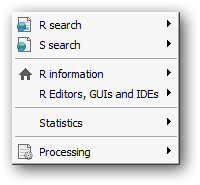
\includegraphics[scale=0.50]{./res/menu_web.png}\\

\begin{scriptsize}\begin{tabularx}{\textwidth}{>{\hsize=0.3\hsize}X>{\hsize=0.7\hsize}X}\\
    \hline
    \textbf{Option} & \textbf{Description} \\
    \hline
    R search & \textit{\htmladdnormallink{See options ...}{\#menu\_web\_rsearch}} \\
    S search & \textit{\htmladdnormallink{See options ...}{\#menu\_web\_ssearch}} \\
    R information & \textit{\htmladdnormallink{See options ...}{\#menu\_web\_rinformation}} \\
    R Editors, GUIs and IDEs & \textit{\htmladdnormallink{See options ...}{\#menu\_web\_rguis}} \\
    Statistics & \textit{\htmladdnormallink{See options ...}{\#menu\_web\_statistics}} \\
    Processing & \textit{\htmladdnormallink{See options ...}{\#menu\_web\_processing}} \\
    \hline
  \end{tabularx}\end{scriptsize}


\hypertarget{menu_web_rsearch}{}
\subsection{R search}
\index{web menu!R search}

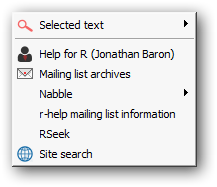
\includegraphics[scale=0.50]{./res/menu_web_rsearch.png}\\

\begin{scriptsize}\begin{tabularx}{\textwidth}{>{\hsize=0.5\hsize}X>{\hsize=0.7\hsize}X}\\
    \hline
    \textbf{Option} & \textbf{Description} \\
    \hline
    Selected text & \textit{\htmladdnormallink{See options ...}{\#menu\_web\_rsearch\_selected}} \\
    Help for R (Jonathan Baron) & Opens URL \htmladdnormallink{Help for R}{http://finzi.psych.upenn.edu/} \\
    Mailing list archives & Opens URL \htmladdnormallink{R mailing lists archive}{http://tolstoy.newcastle.edu.au/R/} \\
    Nabble & \textit{\htmladdnormallink{See options ...}{\#menu\_web\_rsearch\_nabble}} \\
    r-help mailing list information & Opens URL \htmladdnormallink{r-help}{http://www.mail-archive.com/r-help@stat.math.ethz.ch/info.html} \\
    RSeek & Opens URL \htmladdnormallink{R Seek}{http://www.rseek.org/} \\
    Site search & Opens URL \htmladdnormallink{R Site Search}{http://finzi.psych.upenn.edu/search.html} \\
    \hline
  \end{tabularx}\end{scriptsize}


\hypertarget{menu_web_rsearch_selected}{}
\subsubsection{Selected text}\\
\index{web menu!R search selected}


\includegraphics[scale=0.50]{./res/menu_web_rsearch_selected.png}\\

\begin{scriptsize}\begin{tabularx}{\textwidth}{>{\hsize=0.3\hsize}X>{\hsize=0.7\hsize}X}\\
    \hline
    \textbf{Option} & \textbf{Description} \\
    \hline
    Archives & Opens URL \htmladdnormallink{R mailing lists archive}{http://www.googlesyndicatedsearch.com/u/newcastlemaths?q=\&sa=Google+Search} and lists the results associated with the word under the cursor or selected text \\
    Google & Opens URL \htmladdnormallink{Google}{http://www.google.com/webhp?domains=r-project.org\&sitesearch=r-project.org\&btnG=Google+Search} and lists the results associated with the word under the cursor or selected text \\
    Site search & Opens URL \htmladdnormallink{R Site Search}{http://finzi.psych.upenn.edu/search.html} and lists the results associated with the word under the cursor or selected text \\
    \hline
  \end{tabularx}\end{scriptsize}


\newpage
\hypertarget{menu_web_rsearch_nabble}{}
\subsubsection{Nabble}\\

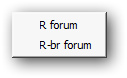
\includegraphics[scale=0.50]{./res/menu_web_rsearch_nabble.png}

\begin{scriptsize}\begin{tabularx}{\textwidth}{>{\hsize=0.3\hsize}X>{\hsize=0.7\hsize}X}\\
    \hline
    \textbf{Option} & \textbf{Description} \\
    \hline
    R forum & Opens URL \htmladdnormallink{R forum}{http://r.789695.n4.nabble.com/} \\
    R-br forum & Opens URL \htmladdnormallink{R-br forum}{http://r-br.2285057.n4.nabble.com/} \\
    \hline
  \end{tabularx}\end{scriptsize}


\hypertarget{menu_web_ssearch}{}
\subsection{S search}

\includegraphics[scale=0.50]{./res/menu_web_ssearch.png}\\
\index{web menu!S search}

\begin{scriptsize}\begin{tabularx}{\textwidth}{>{\hsize=0.3\hsize}X>{\hsize=0.7\hsize}X}\\
    \hline
    \textbf{Option} & \textbf{Description} \\
    \hline
    Selected text & \textit{\htmladdnormallink{See options ...}{\#menu\_web\_search\_selected}} \\
    Mailing list archives & Opens URL \htmladdnormallink{S-News Mailing List Archives}{http://www.biostat.wustl.edu/archives/html/s-news/} \\
    \hline
  \end{tabularx}\end{scriptsize}


\hypertarget{menu_web_ssearch_selected}{}
\subsubsection{Selected text}\\
\index{web menu!S search selected}


\includegraphics[scale=0.50]{./res/menu_web_ssearch_selected.png}\\

\begin{scriptsize}\begin{tabularx}{\textwidth}{>{\hsize=0.3\hsize}X>{\hsize=0.7\hsize}X}\\
    \hline
    \textbf{Option} & \textbf{Description} \\
    \hline
    Archives search & Opens URL \htmladdnormallink{S-news archive search}{http://www.biostat.wustl.edu/archives/cgi-bin/namazu.cgi?query=\&submit=Search\&idxname=s-news} and lists the results associated with the word under the cursor or selected text \\
    \hline
  \end{tabularx}\end{scriptsize}


\hypertarget{menu_web_rinformation}{}
\subsection{R information}
\index{web menu!R information}

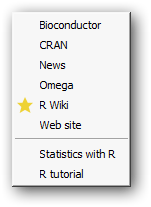
\includegraphics[scale=0.50]{./res/menu_web_rinformation.png}\\

\begin{scriptsize}\begin{tabularx}{\textwidth}{>{\hsize=0.3\hsize}X>{\hsize=0.7\hsize}X}\\
    \hline
    \textbf{Option} & \textbf{Description} \\
    \hline
    Bioconductor & Opens URL \htmladdnormallink{Bioconductor project}{http://www.bioconductor.org/} \\
    CRAN & Opens URL \htmladdnormallink{The Comprehensive R Archive Network}{http://cran.r-project.org/} \\
    News & Opens URL \htmladdnormallink{R News}{http://cran.r-project.org/doc/Rnews/} \\
    Omega & Opens URL \htmladdnormallink{The Omega Project for Statistical Computing}{http://www.omegahat.org/} \\
    R Wiki & Opens URL \htmladdnormallink{R Wiki}{http://wiki.r-project.org/rwiki/doku.php} \\
    Web site & Opens URL \htmladdnormallink{The R Project for Statistical Computing}{http://www.r-project.org/} \\
    Statistical with R & Opens URL \htmladdnormallink{Statistical with R}{http://zoonek2.free.fr/UNIX/48_R/all.html} \\
    R tutorial & Opens URL \htmladdnormallink{R tutorial}{http://www.r-tutor.com/} \\
    \hline
  \end{tabularx}\end{scriptsize}


\hypertarget{menu_web_rguis}{}
\subsection{R Editors, Gui's and IDEs}
\index{web menu!R Editorss}
\index{web menu!R GUIs}
\index{web menu!R IDEs}

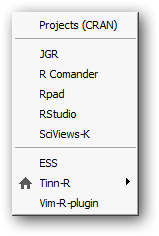
\includegraphics[scale=0.50]{./res/menu_web_rguis.png}\\

\begin{scriptsize}\begin{tabularx}{\textwidth}{>{\hsize=0.3\hsize}X>{\hsize=0.7\hsize}X}\\
    \hline
    \textbf{Option} & \textbf{Description} \\
    \hline
    Projects (CRAN) & Opens URL \htmladdnormallink{R GUI Projects}{http://www.sciviews.org/\_rgui/} \\
    JGR & Opens URL \htmladdnormallink{JGR - Java GUI for R}{http://jgr.markushelbig.org/JGR.html} \\
    R Comander & Opens URL \htmladdnormallink{The R Commander: A Basic-Statistics GUI for R}{http://socserv.socsci.mcmaster.ca/jfox/Misc/Rcmdr/index.html} \\
    Rpad & Opens URL \htmladdnormallink{Rpad home page}{http://www.rpad.org/Rpad/} \\
    RStudio & Opens URL \htmladdnormallink{RStudio}{http://www.rstudio.com/} \\
    SciViews-K & Opens URL \htmladdnormallink{SciViews-K}{http://www.sciviews.org/SciViews-K/} \\
    ESS & Opens URL \htmladdnormallink{Emacs Speaks Statistics (ESS)}{http://ess.r-project.org/} \\
    Tinn-R & \textit{\htmladdnormallink{See options ...}{\#menu\_web\_tinnr}} \\
    Vim-R-plugin & Opens URL \htmladdnormallink{Vim-R-plugin : Plugin to work with R}{http://www.vim.org/scripts/script.php?script\_id=2628} \\
    \hline
  \end{tabularx}\end{scriptsize}


\hypertarget{menu_web_tinnr}{}
\subsection{Tinn-R}
\index{web menu!Tinn-R}

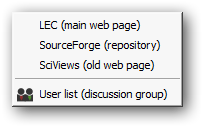
\includegraphics[scale=0.50]{./res/menu_web_tinnr.png}\\


\begin{scriptsize}\begin{tabularx}{\textwidth}{>{\hsize=0.3\hsize}X>{\hsize=0.7\hsize}X}\\
    \hline
    \textbf{Option} & \textbf{Description} \\
    \hline
    LEC (main web page) & Opens URL \htmladdnormallink{LEC}{http://nbcgib.uesc.br/lec/software/editores/tinn-r/en} \\
    SourceForge (repository) & Opens URL \htmladdnormallink{Sourceforge.net Tinn-R}{http://sourceforge.net/projects/tinn-r} \\
    SciViews (old web page) & Opens URL \htmladdnormallink{SciViews Tinn-R}{http://www.sciviews.org/Tinn-R/} \\
    \hline
  \end{tabularx}\end{scriptsize}


\hypertarget{menu_web_statistics}{}
\subsection{Statistics}
\index{web menu!statistics}

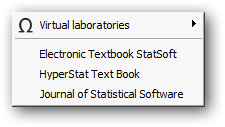
\includegraphics[scale=0.50]{./res/menu_web_statistics.png}\\

\begin{scriptsize}\begin{tabularx}{\textwidth}{>{\hsize=0.5\hsize}X>{\hsize=0.7\hsize}X}\\
    \hline
    \textbf{Option} & \textbf{Description} \\
    \hline
    Virtual laboratories & \textit{\htmladdnormallink{See options ...}{\#menu\_web\_statistics\_virtuallabs}} \\
    Electronic Textbook StatSoft & Opens URL \htmladdnormallink{Electronic Textbook StatSoft}{http://www.statsoft.com/textbook/stathome.html} \\
    HyperStat Text Book & Opens URL \htmladdnormallink{HyperStat Text Book}{http://davidmlane.com/hyperstat/index.html} \\
    Journal of Statistical Software & Opens URL \htmladdnormallink{Journal of Statistical Software}{http://www.jstatsoft.org/} \\
    \hline
  \end{tabularx}\end{scriptsize}


\newpage
\hypertarget{menu_web_statistics_virtuallabs}{}
\subsubsection{Virtual laboratories}\\
\index{web menu!statistics virtual labs}

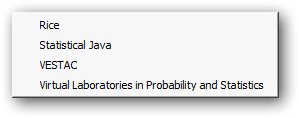
\includegraphics[scale=0.50]{./res/menu_web_statistics_virtuallabs.png}\\

\begin{scriptsize}\begin{tabularx}{\textwidth}{>{\hsize=0.3\hsize}X>{\hsize=0.7\hsize}X}\\
    \hline
    \textbf{Option} & \textbf{Description} \\
    \hline
    Rice & Opens URL \htmladdnormallink{Rice Virtual Lab in Statistics}{http://onlinestatbook.com/rvls.html} \\
    Statistical Java & Opens URL \htmladdnormallink{Statistical Java}{http://www.causeweb.org/repository/statjava/} \\
    VESTAC & Opens URL \htmladdnormallink{Java Applets for Visualization of Statistical Concepts}{http://lstat.kuleuven.be/java/} \\
    Virtual Laboratories in Probability and Statistics & Opens URL \htmladdnormallink{Virtual Laboratories in Probability and Statistics}{http://www.math.uah.edu/stat/} \\
    \hline
  \end{tabularx}\end{scriptsize}


\hypertarget{menu_web_processing}{}
\subsection{Processing}
\index{web menu!processing}

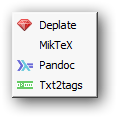
\includegraphics[scale=0.50]{./res/menu_web_processing.png}\\

\begin{scriptsize}\begin{tabularx}{\textwidth}{>{\hsize=0.3\hsize}X>{\hsize=0.7\hsize}X}\\
    \hline
    \textbf{Option} & \textbf{Description} \\
    \hline
    Deplate & Opens URL \htmladdnormallink{Sourceforge.net Deplate}{http://deplate.sourceforge.net/index.php} \\
    MikTeX & Opens URL \htmladdnormallink{MiKTeX project page}{http://miktex.org/} \\
    Pandoc & Opens URL \htmladdnormallink{Pandoc (a universal document converter)}{http://johnmacfarlane.net/pandoc/} \\
    Txt2tags & Opens URL \htmladdnormallink{Txt2tags ONE source, MULTI targets}{http://txt2tags.sourceforge.net/} \\
    \hline
  \end{tabularx}\end{scriptsize}
